%=============================================================================================
%   Criado por Jimi (Willian Bonner) em 29/01/2026
%	Última atualização: 14/03/2026
%   Arquivo final do TCC
%   Versão final
%=============================================================================================

% 1. Pacotes iniciais

\documentclass[12pt, a4paper, openright]{book}
\usepackage[utf8]{inputenc}
\usepackage[T1]{fontenc}
\usepackage[brazilian]{babel}
\usepackage[headsep=1.2cm, top=3cm, bottom=2cm, left=2cm, right=2cm]{geometry}
\usepackage{times}
\usepackage{color}
\usepackage{graphicx}
\usepackage{indentfirst}
\usepackage{multicol}
\usepackage[shortlabels]{enumitem}
\usepackage{subcaption}
\usepackage{emptypage}
\usepackage{tcolorbox}
\usepackage{framed}
\usepackage{etoolbox}
\usepackage{lipsum}
\usepackage{pdflscape}
\usepackage{rotating}

%=============================================================================================
% Pacotes matemáticos e suas configurações
%=============================================================================================

% 1. Pacotes utilizados no código
\usepackage{amsmath, amssymb, amsthm}
\usepackage{mathrsfs}
\usepackage{physics}
\usepackage{newtxmath}
\usepackage{newunicodechar}

% 2. Configuração de "ambientes" matemáticos 

\theoremstyle{definition}
\newtheorem{teo}{Teorema}[section]
\newtheorem{prop}{Proposição}[section]
\newtheorem{Nota}{Notação}[section]
\newtheorem{lema}{Lema}[section]
\newtheorem{cor}{Corolário}[section]
\newtheorem{ex}{Exemplo}[section]
\newtheorem{af}{Afirmação}[section]
\newtheorem{Def}{Definição}[section]
\newtheorem{obs}{Observação}[section]

% 3. Definição de comandos matemáticos

\newcommand{\Ker}{\mathrm{Ker}}
\newcommand{\bb}[1]{\mathbb{#1}}
\newcommand{\tn}[1]{\mathrm{\textbf{#1}}}
\newcommand{\parcial}[2]{\dfrac{\partial #1}{\partial #2}}
\newcommand{\derivada}[2]{\dfrac{d #1}{d #2}}
\newcommand{\dn}[1]{\stackrel{.}{#1}}
\newcommand{\limite}{\displaystyle\lim}
\newcommand{\soma}{\displaystyle\sum}
\newcommand{\tx}[1]{\textrm{#1}}
\newcommand{\N}{\mathbb{N}}
\newcommand{\Z}{\mathbb{Z}}
\newcommand{\Q}{\mathbb{Q}}
\newcommand{\I}{\mathbb{I}}
\newcommand{\R}{\mathbb{R}}
\newcommand{\C}{\mathbb{C}}
\newcommand{\mda}[1]{\left<#1\right>}
\newcommand{\E}{\mathcal{E}}
\newcommand{\Jb}{\mathbf{J}}
\newcommand{\Jf}[1]{\mathbf{J} \qty(#1)}
\newcommand{\sen}[1]{\textrm{sen} \qty(#1)}
\newenvironment{dem}[1][Prova]{\noindent\textbf{#1.} }{\hfill\ \rule{0.5em}{0.5em}}

% 4. Configurações diversas

\let\lambda\uplambda
\newunicodechar{₃}{$_3$}
\DeclareMathSizes{12}{12}{7}{7}

%=============================================================================================
% Configuração da formatação
%
% IMPORTANTE: O titlesec deve ser configurado ANTES do fancyhdr
% Configuração dos títulos antes do fancyhdr
%
%=============================================================================================

% 1. Pacotes utilizados 

\usepackage{titlesec}
\usepackage{caption}

% 2. Configuração dos capítulos

\titleformat{\chapter}[display]
{\centering\normalfont\bfseries\Large}
{\centering\thechapter}
{.5cm}
{\centering}

\titlespacing*{\chapter}{0pt}
{3ex plus 1ex minus .2ex}
{5ex plus .7ex}

% 3. Configuração das seções

\titleformat{\section}[display]
{\centering\normalfont\bfseries\Large}
{\centering\thesection}
{.2cm}
{\centering}

\titlespacing*{\section}{0pt}
{3ex plus 1ex minus .2ex}
{5ex plus .7ex}

% 4. Configuração das subseções

\titleformat{\subsection}[display]
{\centering\normalfont\bfseries\large}
{\centering\thesubsection}
{0.3cm}
{\centering}

\titlespacing*{\subsection}{0pt}
{2.5ex plus 1ex minus .2ex}
{5ex plus .2ex}

% 5. Configuração das legendas das imagens

\DeclareCaptionStyle{semnumero}{labelformat=empty, labelsep=none}
\captionsetup[figure]{format=plain, labelfont=bf, justification=centering, singlelinecheck=false}

% 6. Configurações de numeração

\counterwithin{equation}{section}
\counterwithin{figure}{section}

%=============================================================================================
% Configuração da bibliografia - Estilo ABNT
%=============================================================================================

% 1. Pacotes utilizados

\usepackage[style=abnt]{biblatex}
\addbibresource{assets/referencias/references.bib}

% 2. Configurações da bibliografia

\AtBeginBibliography{\renewbibmacro*{bbx:dashcheck}[2]{#2}}
\AtBeginBibliography{\normalsize}
\setlength{\bibitemsep}{1.0em}

%=============================================================================================
% Configuração dos cabeçalhos - AGORA sim o fancyhdr
%=============================================================================================

% 1. Pacotes utilizados

\usepackage{fancyhdr}

% 2. Configurar os marks ANTES de definir o estilo

\makeatletter

% 2.1 Corrigir os marks para trabalhar com titlesec

\patchcmd{\chapter}{\if@openright\cleardoublepage\else\clearpage\fi}%
{\if@openright\cleardoublepage\else\clearpage\fi\thispagestyle{plain}}{}{}

% 2.2 Definir os marks corretamente

\renewcommand{\chaptermark}[1]{\markboth{\thechapter.\ #1}{}}
\renewcommand{\sectionmark}[1]{\markright{{\thesection.\ #1}}}

% 3. Configurar o estilo da página

\pagestyle{fancy}
\fancyhf{} % Limpa as configurações padrão

% 4. Configurar os cabeçalhos

\fancyhead[LE]{\normalfont\rmfamily\leftmark}  % Capítulo na página par (esquerda)
\fancyhead[RO]{\normalfont\rmfamily\rightmark} % Seção na página ímpar (direita)

% Número da página nas extremidades opostas
\fancyhead[RE,LO]{\normalfont\rmfamily\thepage}

% Definir a espessura da linha (headrule)
\renewcommand{\headrulewidth}{0pt}

% Estilo para páginas em branco (openright)
\fancypagestyle{plain}{%
	\fancyhf{} % Limpa o cabeçalho e rodapé
	\renewcommand{\headrulewidth}{0pt} % Remove a linha
	\fancyfoot[C]{\thepage} % Apenas o número da página no centro
}

%=============================================================================================
% Configurações das referências cruzadas
%=============================================================================================

% 1. Pacotes utilizados
\usepackage{hyperref}

% 2. Configuração do hyperref (DEVE ser o último pacote carregado)
\hypersetup{
	colorlinks=true,
	linkcolor=blue,
	filecolor=magenta,
	urlcolor=red,
	citecolor=blue,
	pdftitle={Modelo para TCCs},
	pdfauthor={Willian Bonner C. Melo}
}

% 3. Comandos personalizados para referências

\newcommand{\eref}[1]{\hyperref[#1]{Equação~(\ref*{#1})}}
\newcommand{\esref}[1]{\hyperref[#1]{Equações~(\ref*{#1})}}
\newcommand{\syref}[1]{\hyperref[#1]{Sistema~(\ref*{#1})}}
\newcommand{\figref}[1]{\hyperref[#1]{Figura~\ref*{#1}}}
\newcommand{\fgsref}[1]{\hyperref[#1]{Figuras~\ref*{#1}}}
\newcommand{\secref}[1]{\hyperref[#1]{Seção~\ref*{#1}}}
\newcommand{\subsecref}[1]{\hyperref[#1]{Subseção~\ref*{#1}}}
\newcommand{\apdref}[1]{\hyperref[#1]{Apêndice:~\nameref*{#1}}}
\newcommand{\dfref}[1]{\hyperref[#1]{Definição~\ref*{#1}}}
\newcommand{\teoref}[1]{\hyperref[#1]{Teorema~\ref*{#1}}}

\begin{document}
	
	\begin{titlepage}%capa e folha de rosto
		\begin{center}
			\Large{\textbf{UNIVERSIDADE FEDERAL DE SERGIPE} \\
				\textbf{CENTRO DE CIÊNCIAS EXATAS E TECNOLOGIA}\\
				\textbf{DEPARTAMENTO DE FÍSICA}}\\
			\vspace{4cm}%Análise de Sistemas Dinâmicos Aplicada a Lasers: Um Estudo das Equações de Taxa e de Maxwell-Bloch
			{\large\textbf{TÍTULO DO SEU TRABALHO}}
			\vfill
			
			\large \textbf{Seu nome}  
			
			\vfill
			\textbf{Orientador:} nome do orientador
			
			\vspace{3cm}
			{\large Cidade, Estado} \\  
			{\large data}  
		\end{center}
	\newpage
	\thispagestyle{empty}
		\begin{center}
			{\large Seu nome}
			\vspace{3cm}
			
			{\large\textbf{TÍTULO DO SEU TRABALHO}}
			\normalsize
			\vspace{4.5cm}
			
			%Aqui você
			\begin{flushright}
				\normalsize
				\begin{minipage}{0.6\textwidth}
					Trabalho de Conclusão de Curso apresentado ao\\
					Departamento de Física da Universidade Federal\\
					de Sergipe como requisito parcial para obtenção\\
					do título de Bacharel em Física.
				\end{minipage}
			\end{flushright}
			
			\vfill
			\textbf{Orientador:} Nome do orientador
			
			\vspace{3cm}
			{\large Cidade, Estado} \\  
			{\large Data}%Talvez 06/03/2026
		\end{center}
	\end{titlepage}
	
	
	\newpage
	\pagenumbering{roman}
	
	% Dedicatória
	\thispagestyle{empty}
	\vspace*{\fill}
	\begin{flushright}
		\textit{Quando você elimia o impossível, o que sobra,\\ por mais improvável que seja, provavelmente é a verdade.}\\\vspace{.3cm}Sherlock Holmes.
	\end{flushright}
	
	%resumo pt-br
	\chapter*{Agradecimentos}
	
		\textbf{Seus agradecimentos}
	
	\newpage
	\chapter*{Resumo}
		
		\textbf{Seu resumo.}
	
	%resumo gringo
	\newpage
	\chapter*{Abstract}
	
		\textbf{Your abstract.}
	
	
	%sumário
	\thispagestyle{empty}
	\hypersetup{linkcolor=black}
	\tableofcontents
	
	
%	\tableofcontents
%	\cleardoublepage
	
	% Lista de figuras/tabelas (opcional)
	\listoffigures
	\hypersetup{linkcolor=blue}
	% Prefácio, Agradecimentos (usando chapter* para não numerar)

		
		
	\cleardoublepage
	
	% ====================
	% MAIN MATTER
	% ====================
	\mainmatter
	
	% Capítulos numerados, centralizados
	\chapter{Introdução}
	
		Esse documento foi disponibilizado caso alguém queria usar como modelo para seu TCC. 
		
	\section{uma imagem}
	
		\begin{figure}[h]
			\centering
			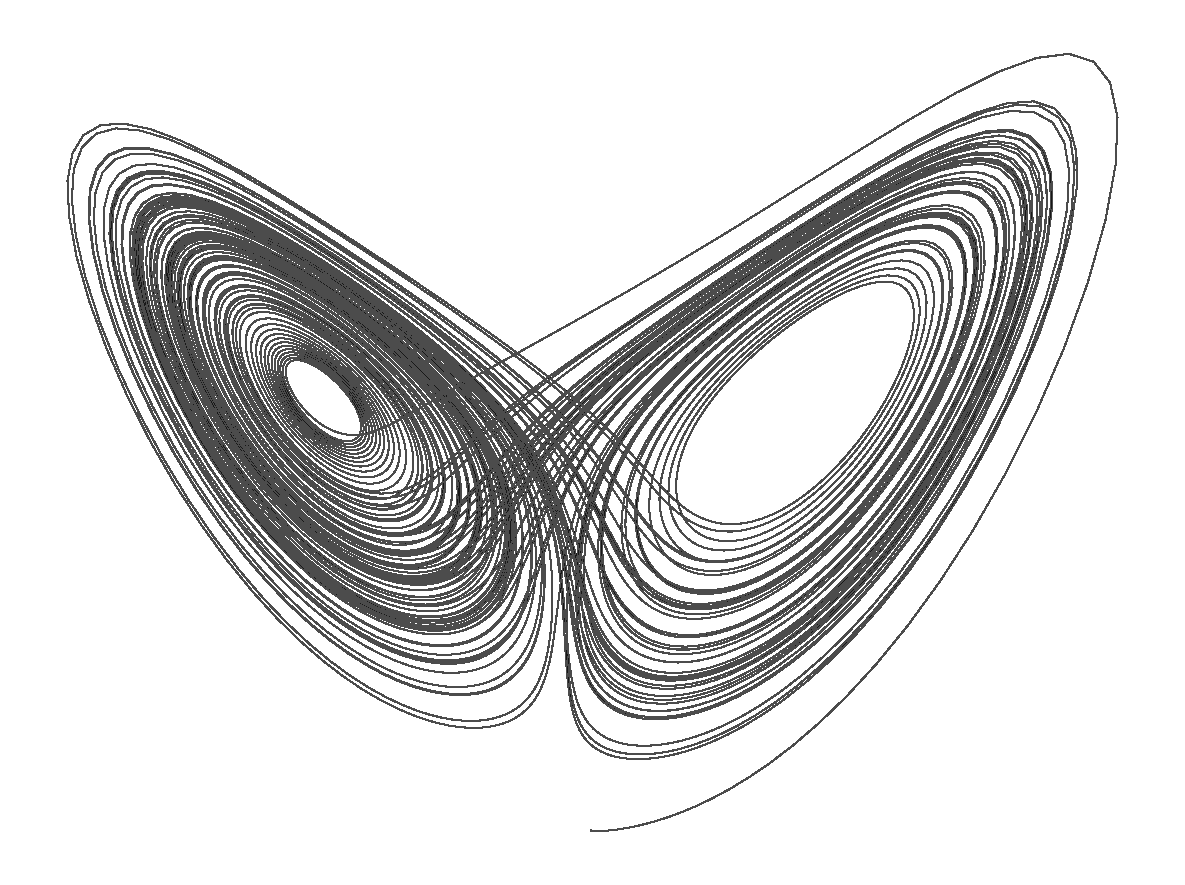
\includegraphics[scale=.6]{assets/images/lz.pdf}
			\caption[Atrator estranho de Lorenz]{Atrator de Lorenz para os parâmetros $\sigma = 10$, $b = \frac{8}{3}$ e $r = 28$.\\\textbf{Fonte:} Imagem gerada pelo autor.}\label{lz01}
		\end{figure}
		
		As referências foram baseadas na ABNT, porém não estão normalizadas pela ABNT, como você pode ver:
		\begin{center}
			A referência \cite{Strogatz_l1}
		\end{center}
	
	\chapter{Fundamentação Teórica}
		
	\chapter{Resultados}
	
	\chapter{Conclusão}
	
	\chapter{Referências}
	
		\printbibliography[heading=none]
	
	\newpage
	\appendix
	
	\chapter{Um apêndice qualquer}\label{ap2}
	
	% Bibliografia
%	\bibliographystyle{plain}
%	\bibliography{referencias}
	
	% Índice remissivo (opcional)
	%\printindex
	
\end{document}